% Created 2024-09-15 Sun 20:05
% Intended LaTeX compiler: pdflatex
\documentclass[12pt]{article}
\usepackage[utf8]{inputenc}
\usepackage[T1]{fontenc}
\usepackage{graphicx}
\usepackage{longtable}
\usepackage{wrapfig}
\usepackage{rotating}
\usepackage[normalem]{ulem}
\usepackage{amsmath}
\usepackage{amssymb}
\usepackage{capt-of}
\usepackage{hyperref}
\usepackage[margin=1in]{geometry} \usepackage{amsmath}
\author{Jason Press}
\date{\today}
\title{Detailed Homework 4}
\hypersetup{
 pdfauthor={Jason Press},
 pdftitle={Detailed Homework 4},
 pdfkeywords={},
 pdfsubject={},
 pdfcreator={Emacs 29.4 (Org mode 9.7.11)}, 
 pdflang={English}}
\begin{document}

\maketitle
\section{Checks}
\label{sec:org43fcb29}

For getting \(\Delta x\) when the sphere starts and stops at the same height, I use the following equation:

\begin{align}
\Delta x = \frac{ v_0^2 }{g}\sin(2\theta)
\end{align}

All of the checks are correct, within a couple fractions of a second. The reason this simulation is not perfectly accurate is the \texttt{time\_step} variable: our simulation is an \emph{approximation} of reality, using a discrete procedural approach to determine the answer. This approach would give a perfect answer if \texttt{time\_step = 0}, but that is not possible. Instead, I approximate it with \texttt{0.01} so the simulation runs in real time. To achieve better agreement with the equations, lower \texttt{time\_step} to even closer to \texttt{0}, such as \texttt{0.00001}. However, this is more costly to run, since the computer has to run more calculations.

The check answers are rounded to the amount of significant figures in the program.
\subsection{\(v_0 = 10 \frac{\text{m}}{\text{s}} \land \theta = 45 ^{\circ}\)}
\label{sec:org1e7fb78}

\begin{align*}
\Delta x = \frac{10^2}{9.81}\sin(2 \cdot 45^{\circ}) \text{m} = 10.19 \text{m}
\end{align*}

The simulation gives 10.32m. While this is not perfectly accurate, it is very close.
\subsection{\(v_0 = 10 \frac{\text{m}}{\text{s}} \land \theta = 90 ^{\circ}\) (straight up)}
\label{sec:orga9787a7}

\begin{align*}
\Delta x = \frac{10^2}{9.81}\sin(2 \cdot 90^{\circ}) \text{m} = 0 \text{m}
\end{align*}

The simulation gives 0.00m, which is the correct answer.
\subsection{\(v_0 = 15 \frac{\text{m}}{\text{s}} \land \theta = 60 ^{\circ}\)}
\label{sec:org6e409c6}

\begin{align*}
\Delta x = \frac{15^2}{9.81}\sin(2 \cdot 60^{\circ}) \text{m} = 19.86 \text{m}
\end{align*}

The simulation gives 19.95m. While this is not perfectly accurate, it is very close.
\subsection{\(v_0 = 10 \frac{\text{m}}{\text{s}} \land \theta = 45 ^{\circ} \land \g = \frac{9.81}{2}\)}
\label{sec:orgd5208f9}

\begin{align*}
\Delta x = \frac{10^2}{\frac{9.81}{2}}\sin(2 \cdot 45^{\circ}) \text{m} = 20.39\text{m}
\end{align*}

The simulation gives 20.51m. While this is not perfectly accurate, it is very close.
\section{Extra Credit: Starting Higher Up}
\label{sec:orgfb9e6cf}

The initial position of the ball in the original program is \texttt{projectile.pos = vector(0, 0, 0)}. By simply taking in a new input \texttt{initial\_height} and making sure it is a non-negative number with a while loop, I can change the initial position to be \texttt{projectile.pos = vector(0, initial\_height, 0)}.

To calculate the new total distance traveled, I can rearrange the kinematic equation in the \(y\) direction for time to give the times when \(y = 0\):

\begin{align} \label{yt}
t = \frac{ -v_0\sin\theta \pm \sqrt{v_0^2\sin^2\theta + 4gy_0}}{2y_0}
\end{align}

Then, I can plug the two answers from Equation \ref{yt} into the kinematic equation in the \(x\) direction to get the following:

\begin{align} \label{x-initial-guess}
x = v_0\cos\theta t = v_0\cos\theta \frac{ -v_0\sin\theta \pm \sqrt{v_0^2\sin^2\theta + 2gy_0}}{-g}
\end{align}

This will give two numbers: one less than or equal to zero, and one greater than or equal to zero. Only caring about the positive displacement, since the ball is traveling forwards in time, I can rewrite Equation \ref{x-initial-guess} to the following:

\begin{align} \label{xt}
x = v_0\cos\theta t = v_0\cos\theta \frac{ v_0\sin\theta + \sqrt{v_0^2\sin^2\theta + 2gy_0}}{g}
\end{align}

The program still suffers the small inaccuracy described in \hyperref[sec:org43fcb29]{checks}.
\subsection{\(v_0 = 10 \frac{\text{m}}{\text{s}} \land \theta = 45 ^{\circ} \land h_0 = 10\text{m}\)}
\label{sec:org0856154}

The output of that equation gives 16.41m. The simulation returns 16.48m.
\subsection{\(v_0 = 15 \frac{\text{m}}{\text{s}} \land \theta = 60 ^{\circ} \land h_0 = 20\text{m}\)}
\label{sec:org14cdb7c}

The output of that equation gives 128.04m. The simulation returns 28.12m.

From these couple examples, it is apparent that the simulation is as consistent with the equations as a discrete approximation can be.
\section{Extra Credit: Maximum Height Coordinates}
\label{sec:org035d2bc}

To achieve this, I added four variables to indicate the maximum \(y\), and only updated them with the current values if the current \(y\) is higher than the maximum recorded \(y\):

\begin{verbatim}
max_x = projectile.pos.x
max_y = projectile.pos.y
min_x_velo = projectile_velocity.x
min_y_velo = projectile_velocity.y

# In the simulation loop

        if max_y < projectile.pos.y:
            max_y = projectile.pos.y
            max_x = projectile.pos.x
            min_x_velo = projectile_velocity.x
            min_y_velo = projectile_velocity.y

        # Display the four variables
\end{verbatim}

To find the minimum acceleration, I just used \(g\), since the only component of acceleration in the simulation is \(g\).

The following equation returns the maximum height when the initial height is equal to the final height:

\begin{align}
y_{max} = \frac{ v_0^2 \sin^2\theta }{ 2g }
\end{align}
\subsection{\(v_0 = 10 \frac{\text{m}}{\text{s}} \land \theta = 45 ^{\circ}\)}
\label{sec:org37b5ea0}

The equation yields a maximum \(y\) of 2.5484. The simulation returns 2.5838.
\subsection{\(v_0 = 15 \frac{\text{m}}{\text{s}} \land \theta = 60 ^{\circ}\)}
\label{sec:org1aa0786}

The equation yields a maximum \(y\) of 8.600. The simulation returns 8.666.

Additionally, for both of these simulations, the maximum \(x\) is half of the horizontal displacement, which is correct for when the initial height is equal to the final height.
\section{Additional Resources}
\label{sec:orgf5b823b}

\href{https://chatgpt.com/share/66e79c20-298c-8004-8420-2adccbdf437f}{Link to ChatGPT conversation.}

\begin{center}
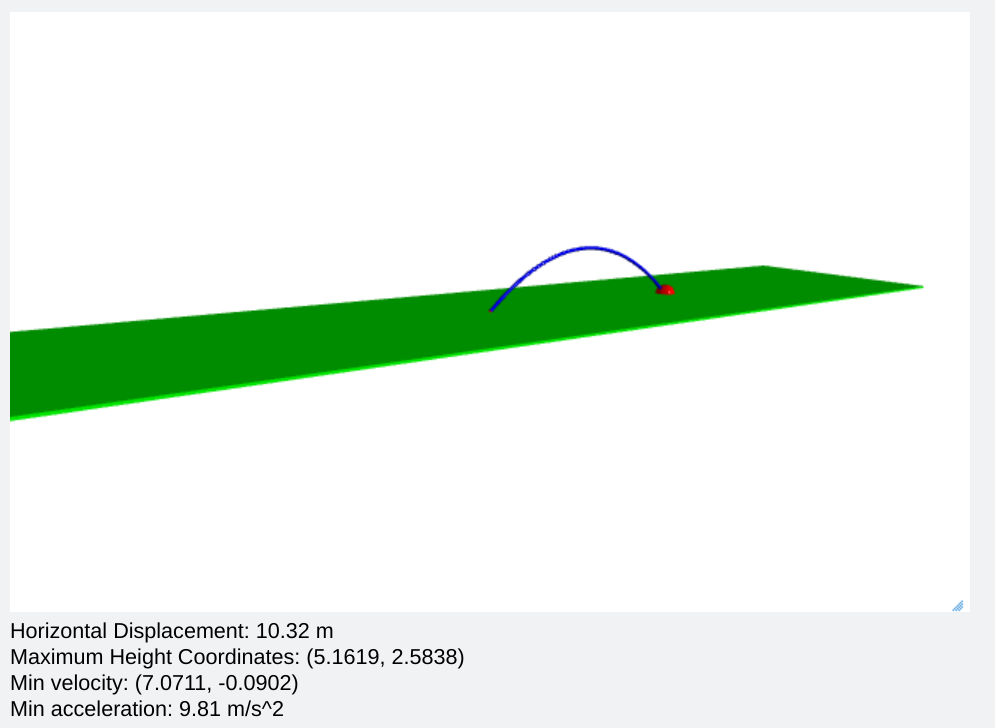
\includegraphics[height=4in]{./10ms.png}
\captionof{figure}{10 meters per second, 45 degrees}
\end{center}

\begin{center}
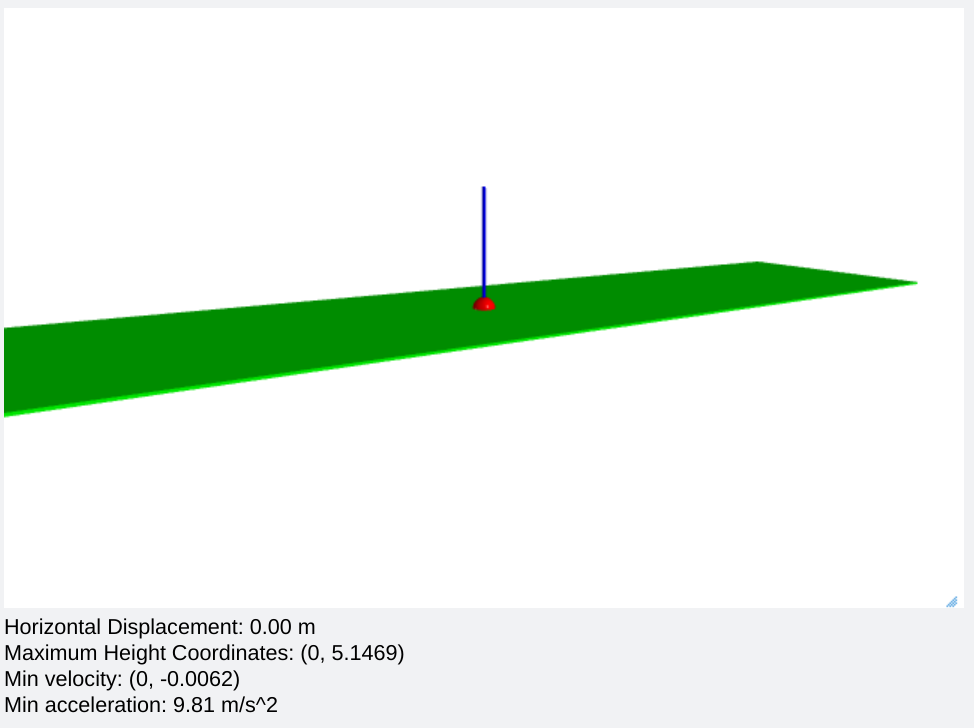
\includegraphics[height=4in]{./straightup.png}
\captionof{figure}{10 meters per second, 90 degrees}
\end{center}

\begin{center}
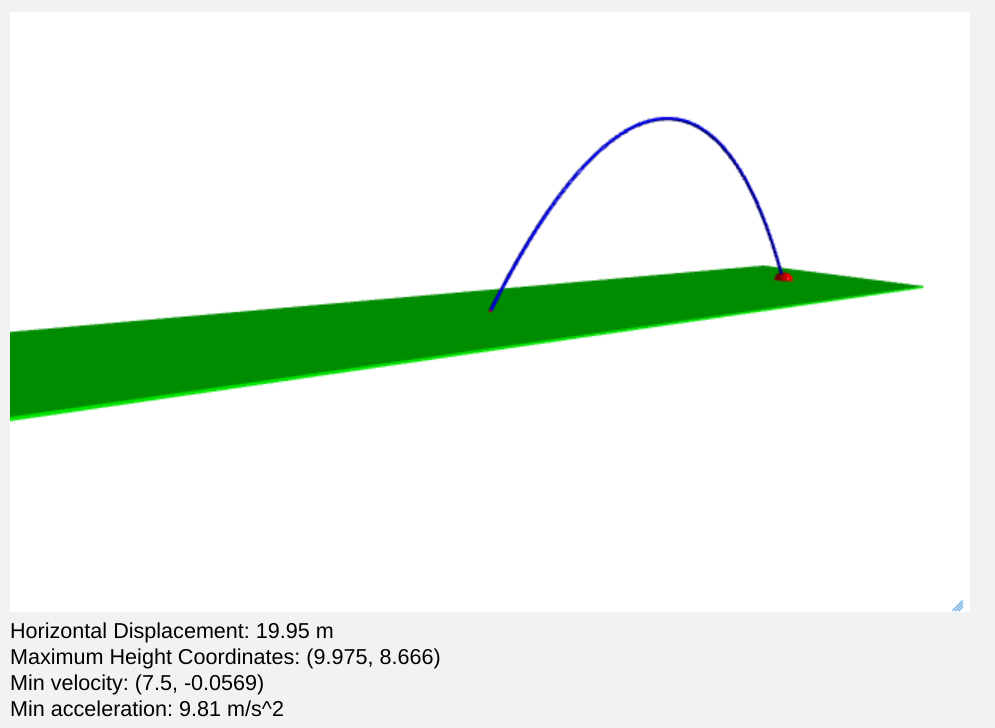
\includegraphics[height=4in]{./15ms.png}
\captionof{figure}{15 meters per second, 60 degrees}
\end{center}

\begin{center}
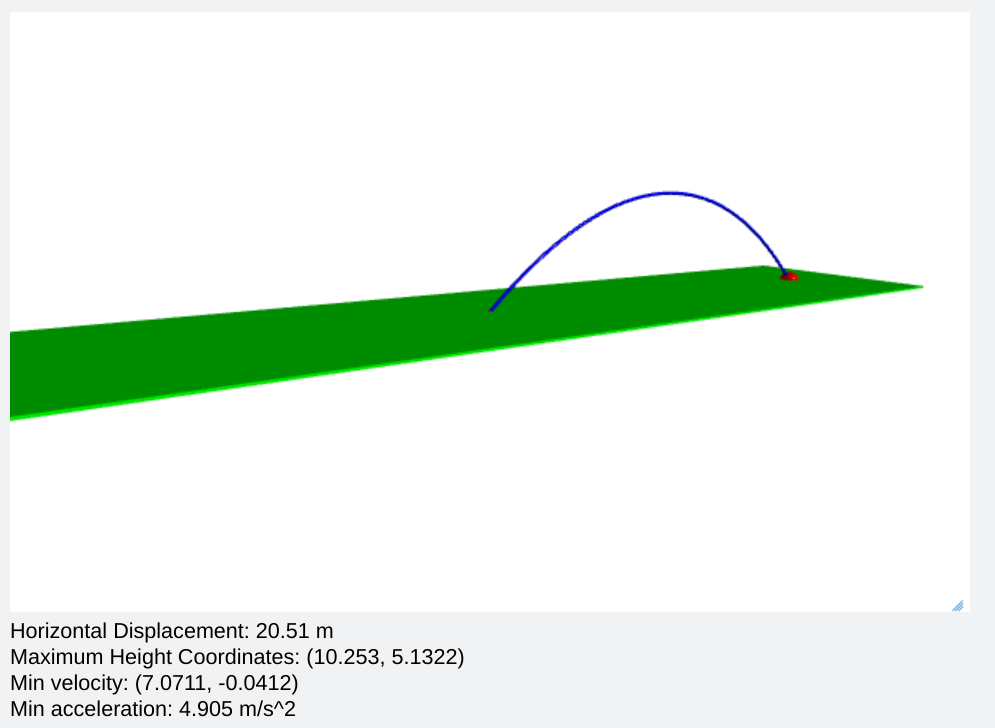
\includegraphics[height=4in]{./halfg.png}
\captionof{figure}{10 meters per second, 45 degrees, half gravity}
\end{center}

\begin{center}
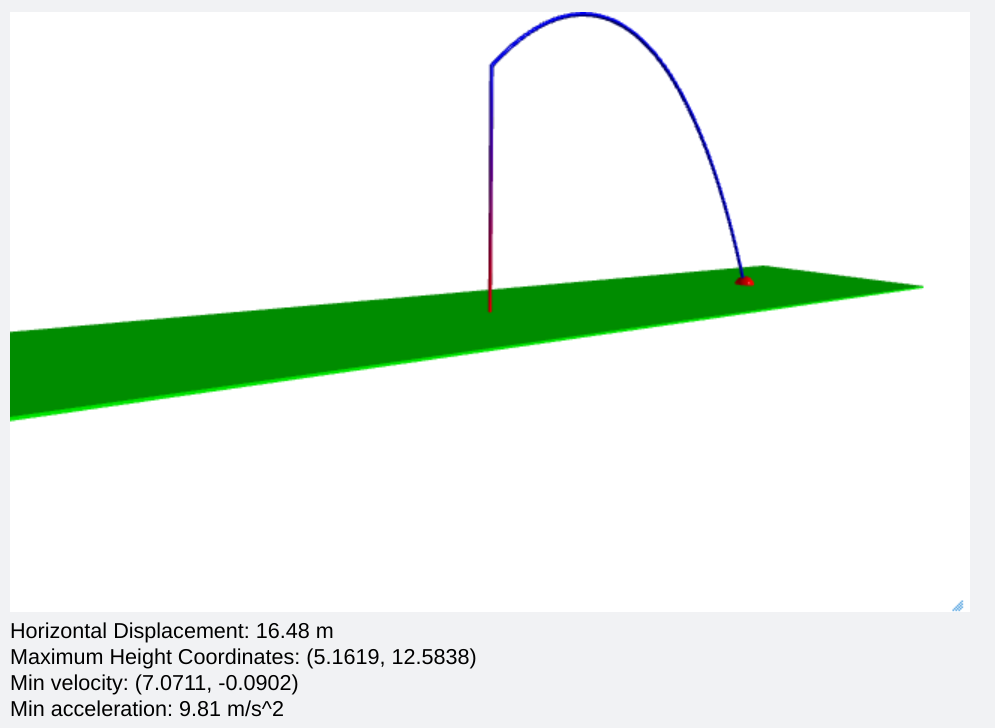
\includegraphics[height=4in]{./10mup.png}
\captionof{figure}{10 meters per second, 45 degrees, 10m up}
\end{center}

\begin{center}
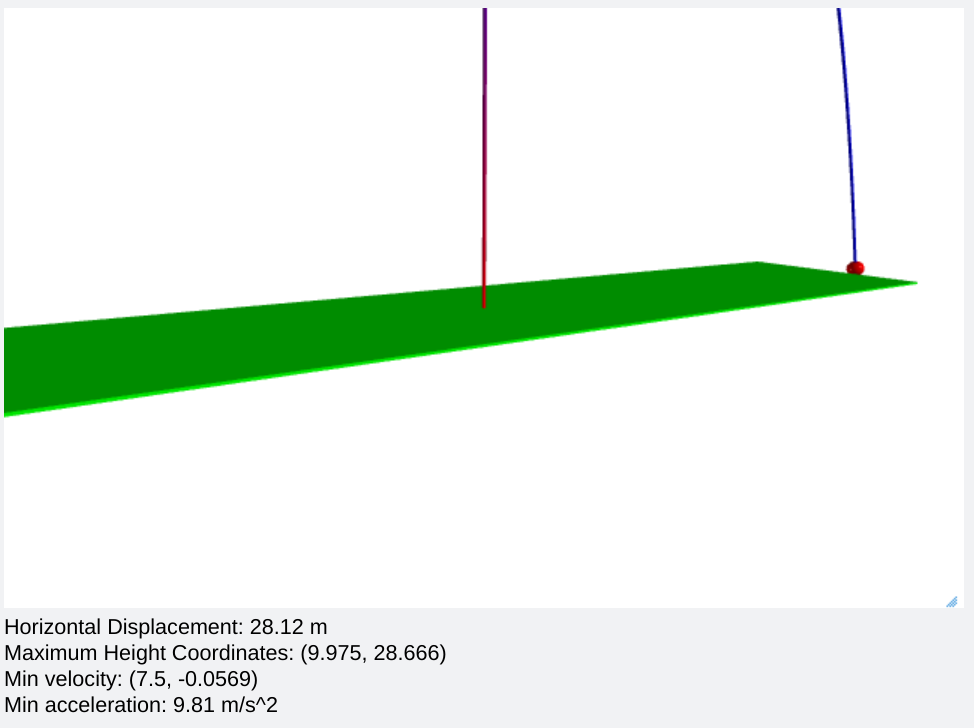
\includegraphics[height=4in]{./20mup.png}
\captionof{figure}{15 meters per second, 60 degrees, 20m up}
\end{center}
\end{document}
